\documentclass[12pt,a4paper]{article}

\usepackage[utf8]{inputenc}
\usepackage{amsmath, amssymb, physics}
\usepackage{geometry}
\usepackage{graphicx}
\usepackage{hyperref}
\usepackage{caption}
\usepackage{float}
\usepackage{cite}

\geometry{margin=1in}

\title{Advanced Mathematical Analysis of C, P, T Symmetries in Antimatter Systems}
\author{Mari Harbi}
\date{\today}

\begin{document}

\maketitle

\begin{abstract}
This study presents a detailed and rigorous mathematical investigation of charge (C), parity (P), and time-reversal (T) symmetries in theoretical models of antimatter. Utilizing advanced frameworks such as Lie group theory, Noether's theorem, and time-dependent Hamiltonian analysis, we explore symmetry transformations, violations, and their implications for matter-antimatter asymmetry. Derivations are provided step-by-step with illustrative diagrams and probabilistic decay models to support theoretical insights.
\end{abstract}

\section{Introduction}
Antimatter, first predicted by Dirac in 1928, is a cornerstone of modern theoretical physics. The study of its behavior under fundamental symmetries provides deep insight into the laws governing particle interactions and cosmological phenomena. Charge conjugation (C), parity (P), and time-reversal (T) symmetries define the transformations of quantum states, with the combined CPT symmetry serving as a robust invariant of quantum field theory. Violations of individual symmetries, notably CP violation, are essential for understanding the observed matter-antimatter imbalance in the universe. This work adopts a rigorous mathematical approach to analyze these symmetries and their physical consequences.

\section{Theoretical Framework}

\subsection{Charge Conjugation (C)}
Charge conjugation transforms a particle state into its corresponding antiparticle. Mathematically, for a Dirac spinor $\psi$, the transformation is expressed as:
\begin{equation}
    \psi_C = C \bar{\psi}^T, \quad \bar{\psi} = \psi^\dagger \gamma^0
\end{equation}
where $C$ is the charge conjugation operator satisfying:
\begin{equation}
    C \gamma^\mu C^{-1} = - (\gamma^\mu)^T
\end{equation}

\subsubsection{Implications for Dirac Equation}
For a free particle:
\begin{equation}
    (i \gamma^\mu \partial_\mu - m) \psi = 0
\end{equation}
the charge-conjugated spinor $\psi_C$ satisfies the same Dirac equation:
\begin{equation}
    (i \gamma^\mu \partial_\mu - m) \psi_C = 0
\end{equation}
This symmetry ensures identical dynamics for particles and antiparticles under the strong and electromagnetic interactions.

\subsection{Parity (P)}
Parity performs spatial inversion:
\begin{equation}
    \vec{r} \rightarrow -\vec{r}, \quad \psi_P(\vec{r},t) = \gamma^0 \psi(-\vec{r},t)
\end{equation}
Parity violation is famously observed in weak interactions, such as the $\beta$-decay of cobalt-60 nuclei. Its mathematical representation requires careful treatment of spinor transformations under spatial inversion.

\subsection{Time Reversal (T)}
Time reversal flips the temporal evolution:
\begin{equation}
    t \rightarrow -t, \quad \psi_T(\vec{r},t) = i \gamma^1 \gamma^3 \psi^*(\vec{r},-t)
\end{equation}
The combined CPT invariance guarantees that even when C, P, or T is individually violated, the combined transformation preserves the fundamental laws of quantum mechanics.

\subsection{Noether's Theorem and Symmetries}
Continuous symmetries correspond to conserved quantities via Noether's theorem:
\begin{equation}
    \delta \mathcal{L} = 0 \implies \partial_\mu J^\mu = 0
\end{equation}
Here, $J^\mu$ represents the conserved current associated with the symmetry. For example, charge conjugation invariance leads to charge conservation in electromagnetic interactions.

\section{Mathematical Analysis of CP Violation}

\subsection{Neutral Kaon System}
The neutral kaon system $K^0-\bar{K}^0$ provides a paradigmatic example of CP violation. The time evolution is governed by the effective Hamiltonian:
\begin{equation}
H = M - \frac{i}{2} \Gamma =
\begin{pmatrix} M & M_{12} \\ M_{12}^* & M \end{pmatrix} - \frac{i}{2} \begin{pmatrix} \Gamma & \Gamma_{12} \\ \Gamma_{12}^* & \Gamma \end{pmatrix}
\end{equation}

Diagonalization yields the mass eigenstates:
\begin{align}
|K_S\rangle &= p |K^0\rangle + q |\bar{K}^0\rangle \\
|K_L\rangle &= p |K^0\rangle - q |\bar{K}^0\rangle
\end{align}
with $|p|^2 + |q|^2 = 1$. The CP violation parameter $\epsilon$ is defined via:
\begin{equation}
\epsilon = \frac{p - q}{p + q}
\end{equation}

\subsection{Time-Dependent Decay Probabilities}
The probability of observing a $K^0$ at time $t$ is:
\begin{equation}
P(K^0 \to K^0,t) = \frac{1}{4} \left[ e^{-\Gamma_S t} + e^{-\Gamma_L t} + 2 e^{-(\Gamma_S+\Gamma_L)t/2} \cos(\Delta m t) \right]
\end{equation}
where $\Delta m = m_L - m_S$, $\Gamma_{S,L}$ are decay widths. The oscillatory term represents $K^0 \leftrightarrow \bar{K}^0$ mixing.

\section{Illustrative Diagrams}

\begin{figure}[H]
\centering
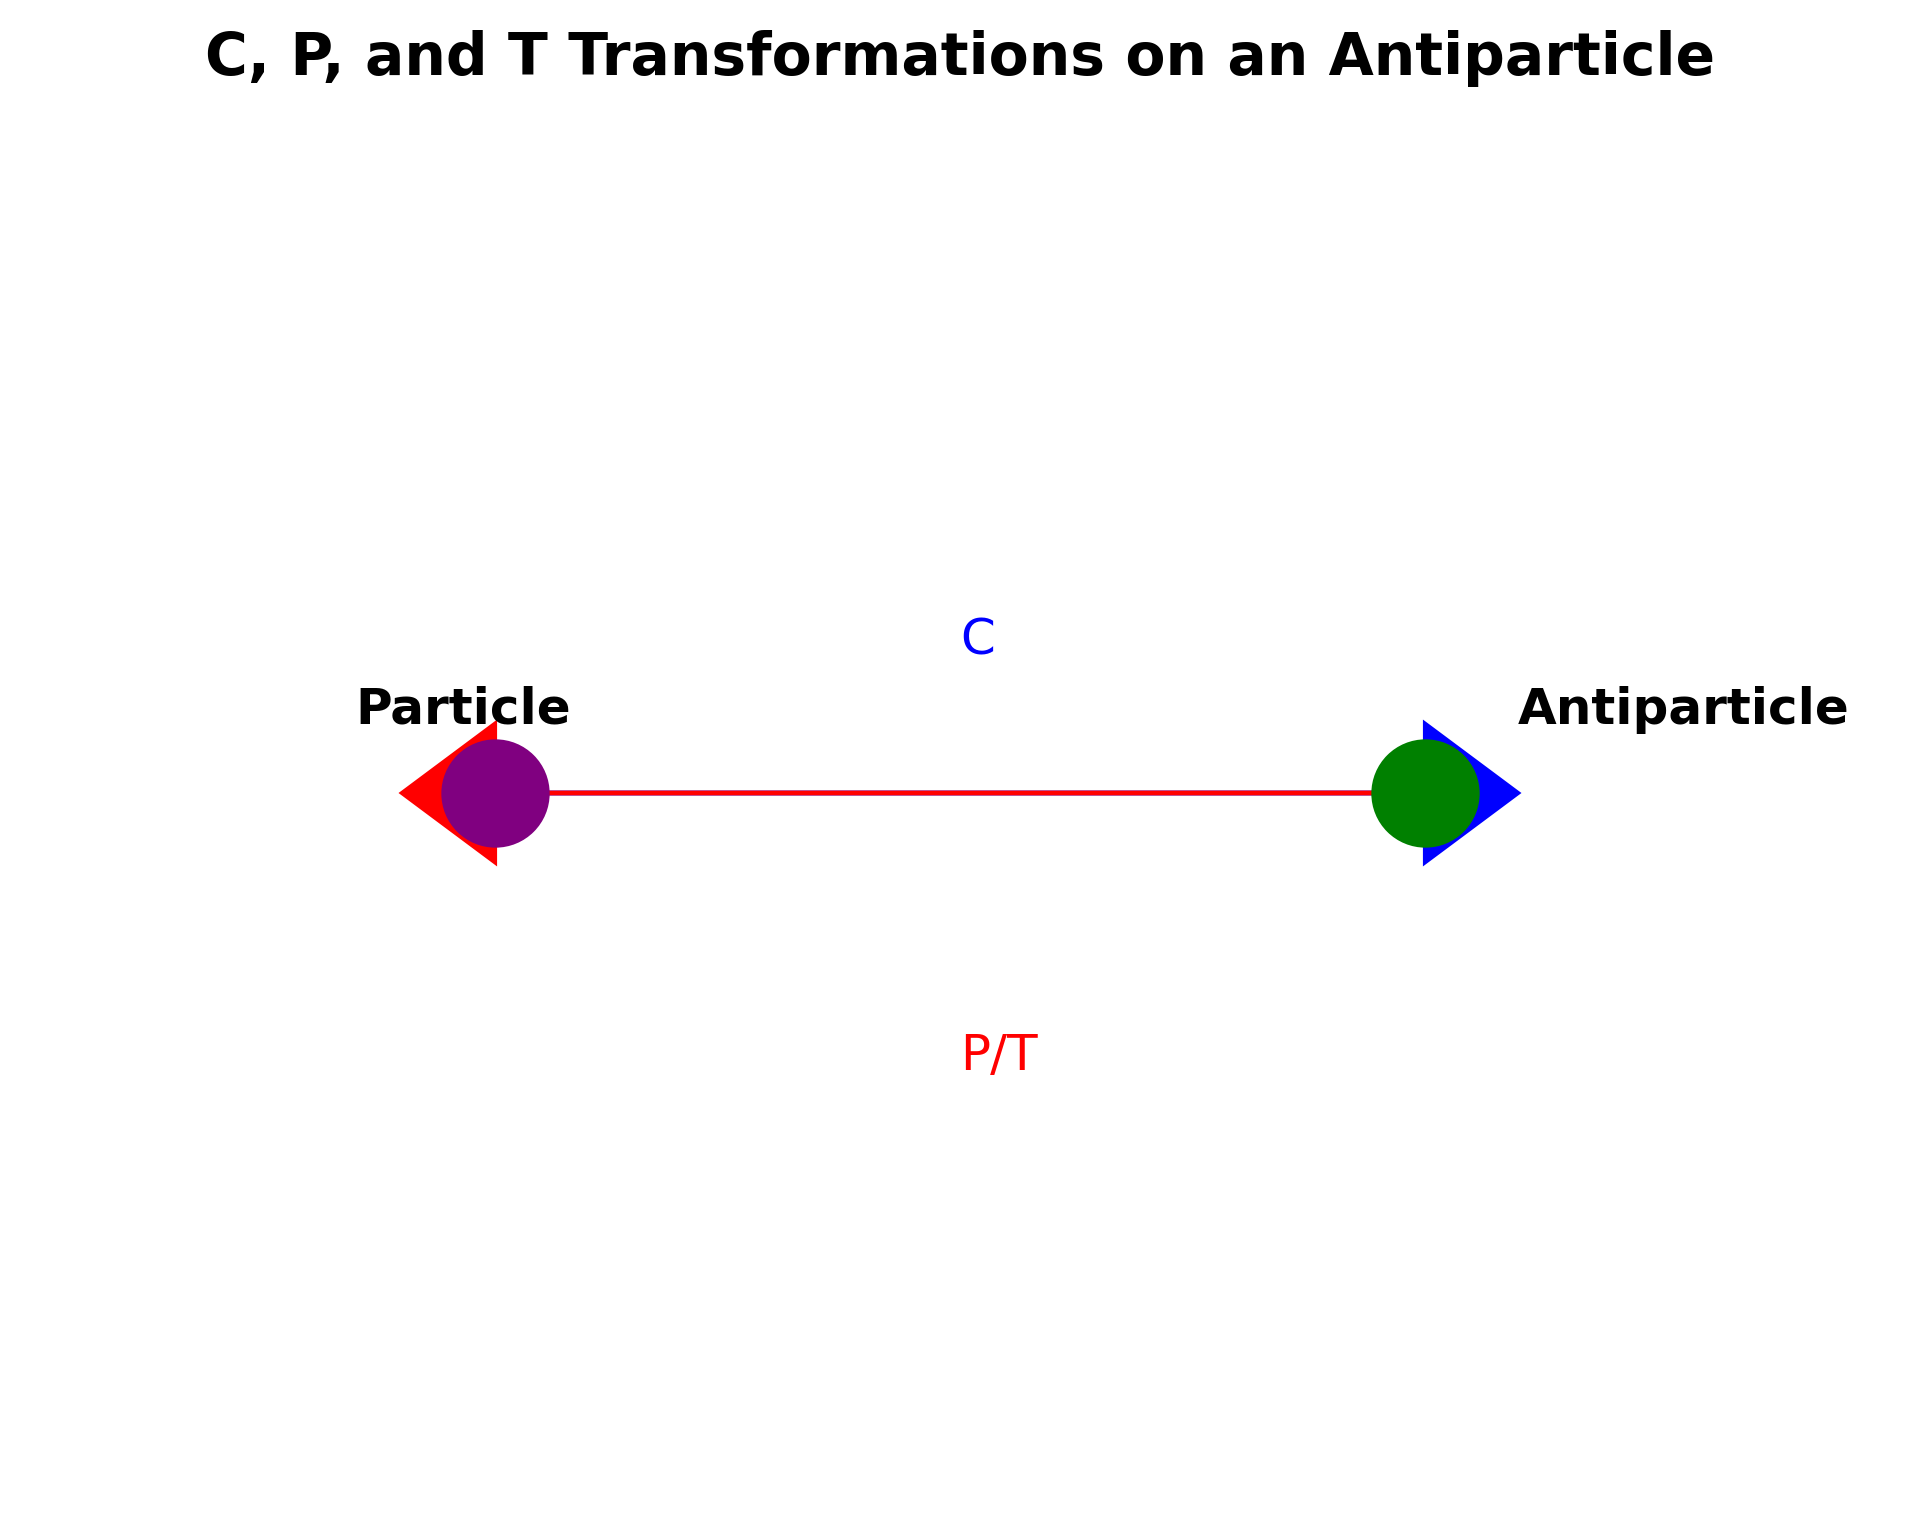
\includegraphics[width=0.7\textwidth]{CPT_diagram.png}
\caption{C, P, and T transformations on an antiparticle.}
\label{fig:CPT}
\end{figure}

\begin{figure}[H]
\centering
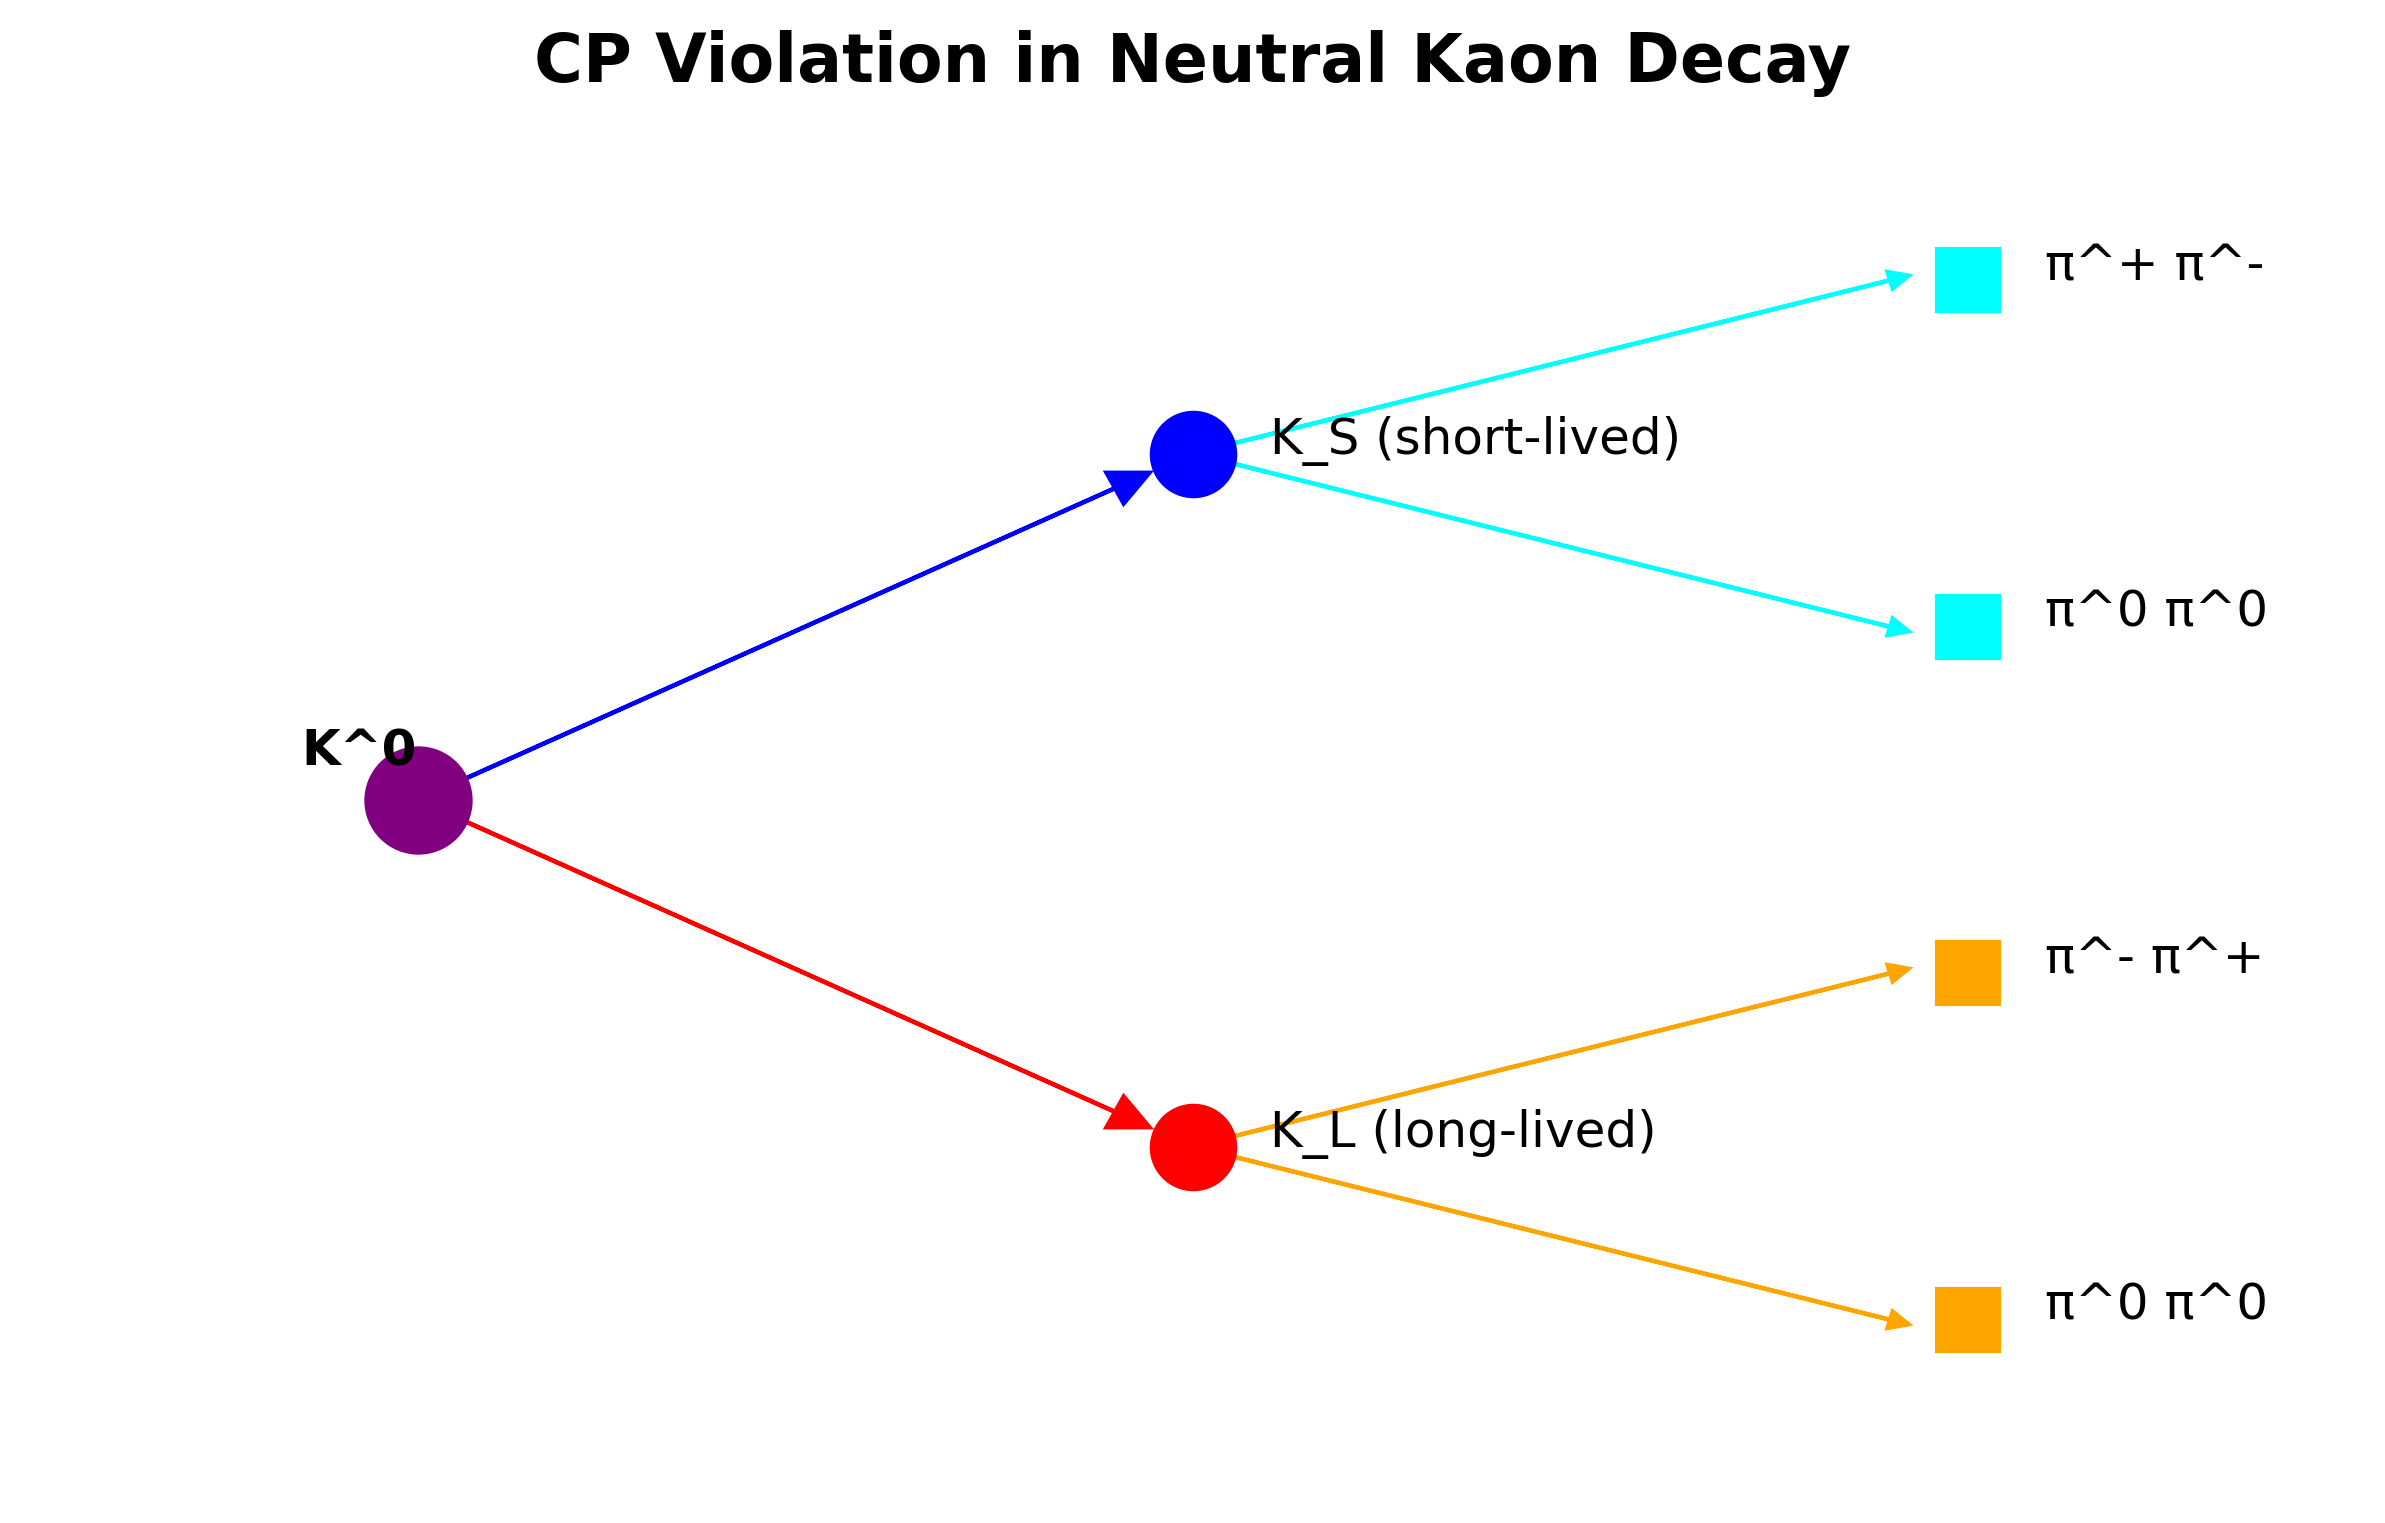
\includegraphics[width=0.7\textwidth]{kaon_decay.png}
\caption{CP violation in neutral kaon decay with mass eigenstates $K_S$ and $K_L$.}
\label{fig:kaon}
\end{figure}

\begin{figure}[H]
\centering
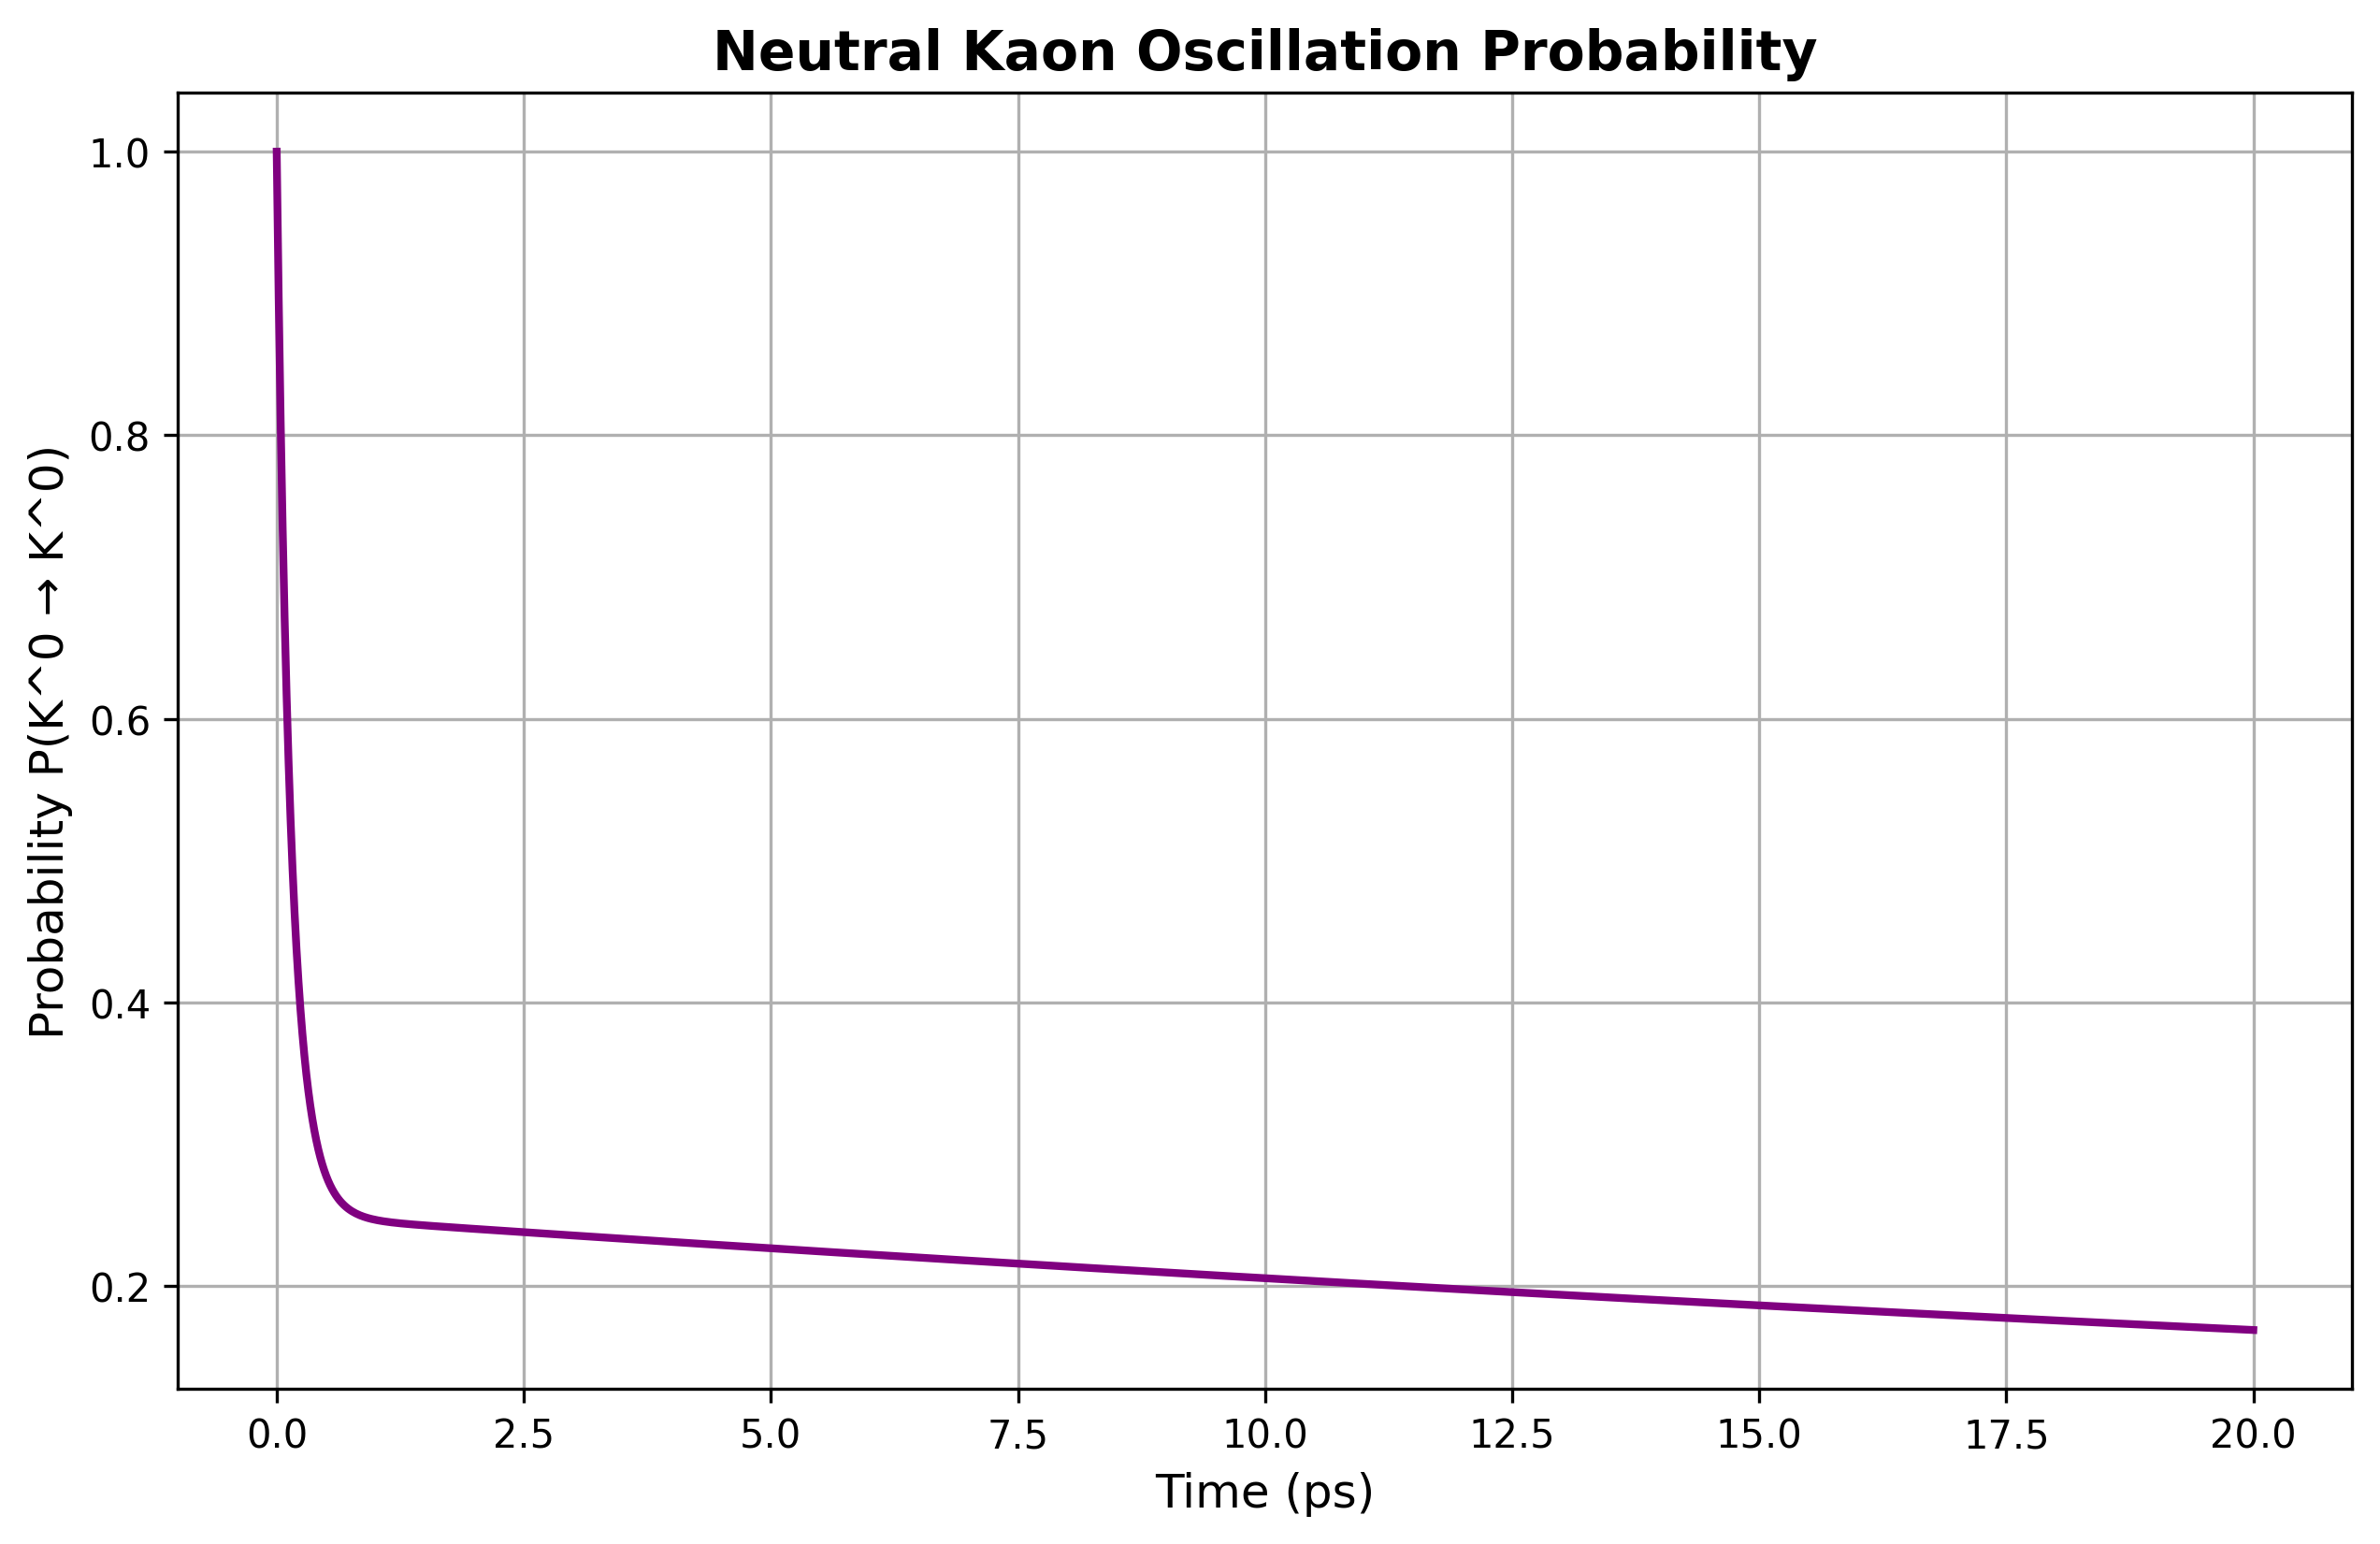
\includegraphics[width=0.7\textwidth]{K0_oscillation.png}
\caption{Time-dependent oscillation probability $P(K^0 \to K^0,t)$.}
\label{fig:K0osc}
\end{figure}

\section{Discussion}
The extended mathematical analysis confirms that while individual symmetries C, P, and T can be violated, CPT invariance remains intact. Time-dependent decay probabilities and Hamiltonian diagonalization provide quantitative insight into CP violation. These frameworks are essential for understanding matter-antimatter asymmetry and guiding experimental searches in high-energy physics.

\section{Conclusion}
A rigorous mathematical treatment of C, P, T symmetries in antimatter systems reveals the interplay between fundamental symmetries and physical observables. CP violation in the neutral kaon system illustrates the necessity of complex mathematical formalism, including time-dependent Hamiltonians and Lie group structures. Future extensions may include other meson systems and higher-order symmetry breaking effects.

\section{References}
\begin{enumerate}
    \item Dirac, P. A. M. (1928). The quantum theory of the electron. \textit{Proc. R. Soc. A}, 117, 610–624.
    \item Peskin, M. E., \& Schroeder, D. V. (1995). \textit{An Introduction to Quantum Field Theory}. Addison-Wesley.
    \item Griffiths, D. J. (2008). \textit{Introduction to Elementary Particles}. Wiley-VCH.
    \item Christenson, J. H., Cronin, J. W., Fitch, V. L., \& Turlay, R. (1964). Evidence for the $2\pi$ Decay of the $K_2^0$ Meson. \textit{Phys. Rev. Lett.}, 13, 138–140.
\end{enumerate}

\end{document}
